% Options for packages loaded elsewhere
\PassOptionsToPackage{unicode}{hyperref}
\PassOptionsToPackage{hyphens}{url}
\documentclass[
  ignorenonframetext,
]{beamer}
\newif\ifbibliography
\usepackage{pgfpages}
\setbeamertemplate{caption}[numbered]
\setbeamertemplate{caption label separator}{: }
\setbeamercolor{caption name}{fg=normal text.fg}
\beamertemplatenavigationsymbolsempty
% remove section numbering
\setbeamertemplate{part page}{
  \centering
  \begin{beamercolorbox}[sep=16pt,center]{part title}
    \usebeamerfont{part title}\insertpart\par
  \end{beamercolorbox}
}
\setbeamertemplate{section page}{
  \centering
  \begin{beamercolorbox}[sep=12pt,center]{section title}
    \usebeamerfont{section title}\insertsection\par
  \end{beamercolorbox}
}
\setbeamertemplate{subsection page}{
  \centering
  \begin{beamercolorbox}[sep=8pt,center]{subsection title}
    \usebeamerfont{subsection title}\insertsubsection\par
  \end{beamercolorbox}
}
% Prevent slide breaks in the middle of a paragraph
\widowpenalties 1 10000
\raggedbottom
\AtBeginPart{
  \frame{\partpage}
}
\AtBeginSection{
  \ifbibliography
  \else
    \frame{\sectionpage}
  \fi
}
\AtBeginSubsection{
  \frame{\subsectionpage}
}
\usepackage{iftex}
\ifPDFTeX
  \usepackage[T1]{fontenc}
  \usepackage[utf8]{inputenc}
  \usepackage{textcomp} % provide euro and other symbols
\else % if luatex or xetex
  \usepackage{unicode-math} % this also loads fontspec
  \defaultfontfeatures{Scale=MatchLowercase}
  \defaultfontfeatures[\rmfamily]{Ligatures=TeX,Scale=1}
\fi
\usepackage{lmodern}
\ifPDFTeX\else
  % xetex/luatex font selection
\fi
% Use upquote if available, for straight quotes in verbatim environments
\IfFileExists{upquote.sty}{\usepackage{upquote}}{}
\IfFileExists{microtype.sty}{% use microtype if available
  \usepackage[]{microtype}
  \UseMicrotypeSet[protrusion]{basicmath} % disable protrusion for tt fonts
}{}
\makeatletter
\@ifundefined{KOMAClassName}{% if non-KOMA class
  \IfFileExists{parskip.sty}{%
    \usepackage{parskip}
  }{% else
    \setlength{\parindent}{0pt}
    \setlength{\parskip}{6pt plus 2pt minus 1pt}}
}{% if KOMA class
  \KOMAoptions{parskip=half}}
\makeatother
\usepackage{graphicx}
\makeatletter
\newsavebox\pandoc@box
\newcommand*\pandocbounded[1]{% scales image to fit in text height/width
  \sbox\pandoc@box{#1}%
  \Gscale@div\@tempa{\textheight}{\dimexpr\ht\pandoc@box+\dp\pandoc@box\relax}%
  \Gscale@div\@tempb{\linewidth}{\wd\pandoc@box}%
  \ifdim\@tempb\p@<\@tempa\p@\let\@tempa\@tempb\fi% select the smaller of both
  \ifdim\@tempa\p@<\p@\scalebox{\@tempa}{\usebox\pandoc@box}%
  \else\usebox{\pandoc@box}%
  \fi%
}
% Set default figure placement to htbp
\def\fps@figure{htbp}
\makeatother
\setlength{\emergencystretch}{3em} % prevent overfull lines
\providecommand{\tightlist}{%
  \setlength{\itemsep}{0pt}\setlength{\parskip}{0pt}}
\usepackage{bookmark}
\IfFileExists{xurl.sty}{\usepackage{xurl}}{} % add URL line breaks if available
\urlstyle{same}
\hypersetup{
  hidelinks,
  pdfcreator={LaTeX via pandoc}}

\author{\texorpdfstring{}{}}
\date{}

\begin{document}

\begin{frame}{The Four Levels of Monetary Vision and Generation}
\protect\phantomsection\label{the-four-levels-of-monetary-vision-and-generation}
Blake maps this escalating socioeconomic and spiritual entropy against
his definitive epistemological concept: the \textbf{Four Levels of
Vision}. This paradigm directly traces the evolution of British monetary
architectures, moving from calculation, through generative (but
unstable) tension, to the ultimate requirement for an overarching
qualitative human integration (as explored further under
\href{04a_illuminated_nonduality.md\#illuminated-nonduality-and-the-fourfold-vision}{Illuminated
Nonduality}). Northrop Frye's foundational elucidation in \emph{Fearful
Symmetry} (1947) establishes that Blake's Fourfold Vision represents not
merely a poetic conceit but a complete philosophical telos: imaginative
creativity operating as a living, breathing power that restores the
fractured human form {[}@frye1947fearful{]}.

\begin{block}{Single Vision (Ulro): Monometallism and Fiat}
\protect\phantomsection\label{single-vision-ulro-monometallism-and-fiat}
The lowest perceptual state in Blake's cosmology is \textbf{Ulro}
(\emph{Single Vision}). Dominated strictly by empirical measurement and
atomistic isolation, it is a realm of spiritual death---what Blake
describes as ``Newtons sleep,'' the stupor of pure quantification. As
Susanne Sklar notes, ``In Ulro, that which can't be expressed
quantitatively does not exist'' {[}@sklar2011blake{]}. In monetary
mechanics, \emph{Single Vision} equates identically to strict
Monometallism---the Urizenic fetishization of a single currency vector
(Gold) serving as an inflexible standard (see the 1816 Regression in
\href{04b_coinage_act_1816.md\#the-1816-coinage-act-as-topological-regression}{the
Coinage Act analysis}). The 1816 Coinage Act, which legally restricted
silver to token coinage with a 40-shilling legal tender limit,
constitutes the legislative realization of Ulro: the elimination of
duality and generative tension in favor of a monistic, reductionist
finality. Ulro is also the state of unbacked fiat paper from 1797---a
disconnected void where the Bank of England's notes, backed by reserves
of only £1,086,170 against over £10 million in circulation, constituted
a semiotic void {[}@clapham1944bank{]}. It enforces total reductionism,
severing spiritual context and dismissing any human value that cannot be
weighed on capitalist scales or entered into a ledger.
\end{block}

\begin{block}{Twofold Vision (Generation): Bimetallism}
\protect\phantomsection\label{twofold-vision-generation-bimetallism}
Escaping the void of Ulro leads to \textbf{Generation} (\emph{Twofold
Vision}). As documented, the Bimetallic standard is the historical
instantiation of Twofold Vision (see \hyperlink{fig-alchemy}{the
Harmonograph}). It is a realm of biological and economic reproduction,
deeply meta-stable, and prone to the unceasing arbitrage of Gresham's
Law. It is a site of suffering and labor, but nevertheless a vastly
superior state to Ulro: it acknowledges duality, tension, and relative
interaction over the violence of geometric singularity. Silver and Gold
exist in a dynamic, albeit precarious, relationship---bound by Newton's
1:15.21 ratio yet perpetually strained by international market forces
that valued silver more highly abroad. This is the productive but
agonizing state of human existence: the alchemical marriage of Sol and
Luna that Del Mar identifies as the sacred foundation of all legitimate
coinage {[}@delmar1895history{]}. The instability is not a flaw but a
feature---it is the generative friction of two irreducible principles in
dialogue, the very condition of creative evolution.
\end{block}

\begin{block}{Threefold Vision (Beulah): The Affective Threshold}
\protect\phantomsection\label{threefold-vision-beulah-the-affective-threshold}
Above Generation lies \textbf{Beulah} (\emph{Threefold Vision}), the
realm of emotional insight and intuitive apprehension. In monetary
terms, Beulah represents the fleeting historical moments when economic
policy briefly served human flourishing rather than extractive
accumulation---periods of relative prosperity and social cohesion that
exist precariously between the grinding mechanisms of Urizenic finance.
Beulah is, in Blake's cosmology, a necessary way-station, a ``married
land'' of rest and restoration, but one that cannot sustain itself
indefinitely without ascending into the full creative synthesis of Eden.
\end{block}

\begin{block}{Fourfold Vision (Eden): The Prophetic Assertion}
\protect\phantomsection\label{fourfold-vision-eden-the-prophetic-assertion}
In \emph{Jerusalem}, the prophetic artisan Los rejects both the void of
Ulro and the mere passive calculation of financial ratios found in
Generation (the 1-fold and 2-fold quantification) with an operational
doctrine:

\begin{quote}
``I must Create a System, or be enslav'd by another Mans / I will not
Reason \& Compare: my business is to Create'' (\emph{Jerusalem}, Plate
10, lines 20--21; Erdman p.~153) {[}@erdman1988complete{]}
\end{quote}

This decree is a direct philosophical rebuff to the bimetallic
arbitrageur who exists only to ``Reason \& Compare'' the Gresham Entropy
Gap---calculating the exact moment when the silver-to-gold ratio across
the channel offers a risk-free margin. It is also, at a generic level, a
rejection of the foundational axiom of classical political economy: that
rational self-interest, expressed through price signals and arbitrage,
constitutes the highest form of social coordination. Blake insists that
the \emph{minute particular}---the irreducible, non-fungible quality of
individual human experience---cannot be captured by any system of
relative prices. As Makdisi argues, Blake's anti-capitalism is not a
sentimental nostalgia for pre-industrial life but a rigorous,
philosophically grounded rejection of the entire framework of commodity
exchange {[}@makdisi2003william{]}. Through Los's roaring furnaces,
Blake asserts the absolute necessity of advancing beyond quantitative
mechanics. He demands a leap into the qualitative synthesis of the
\emph{Threefold} (emotional/affectionate) and \emph{Fourfold}
(Edenic/imaginative) states, where real value is birthed in artistic and
spiritual creation rather than through financial extraction.

\begin{figure}
\centering
\pandocbounded{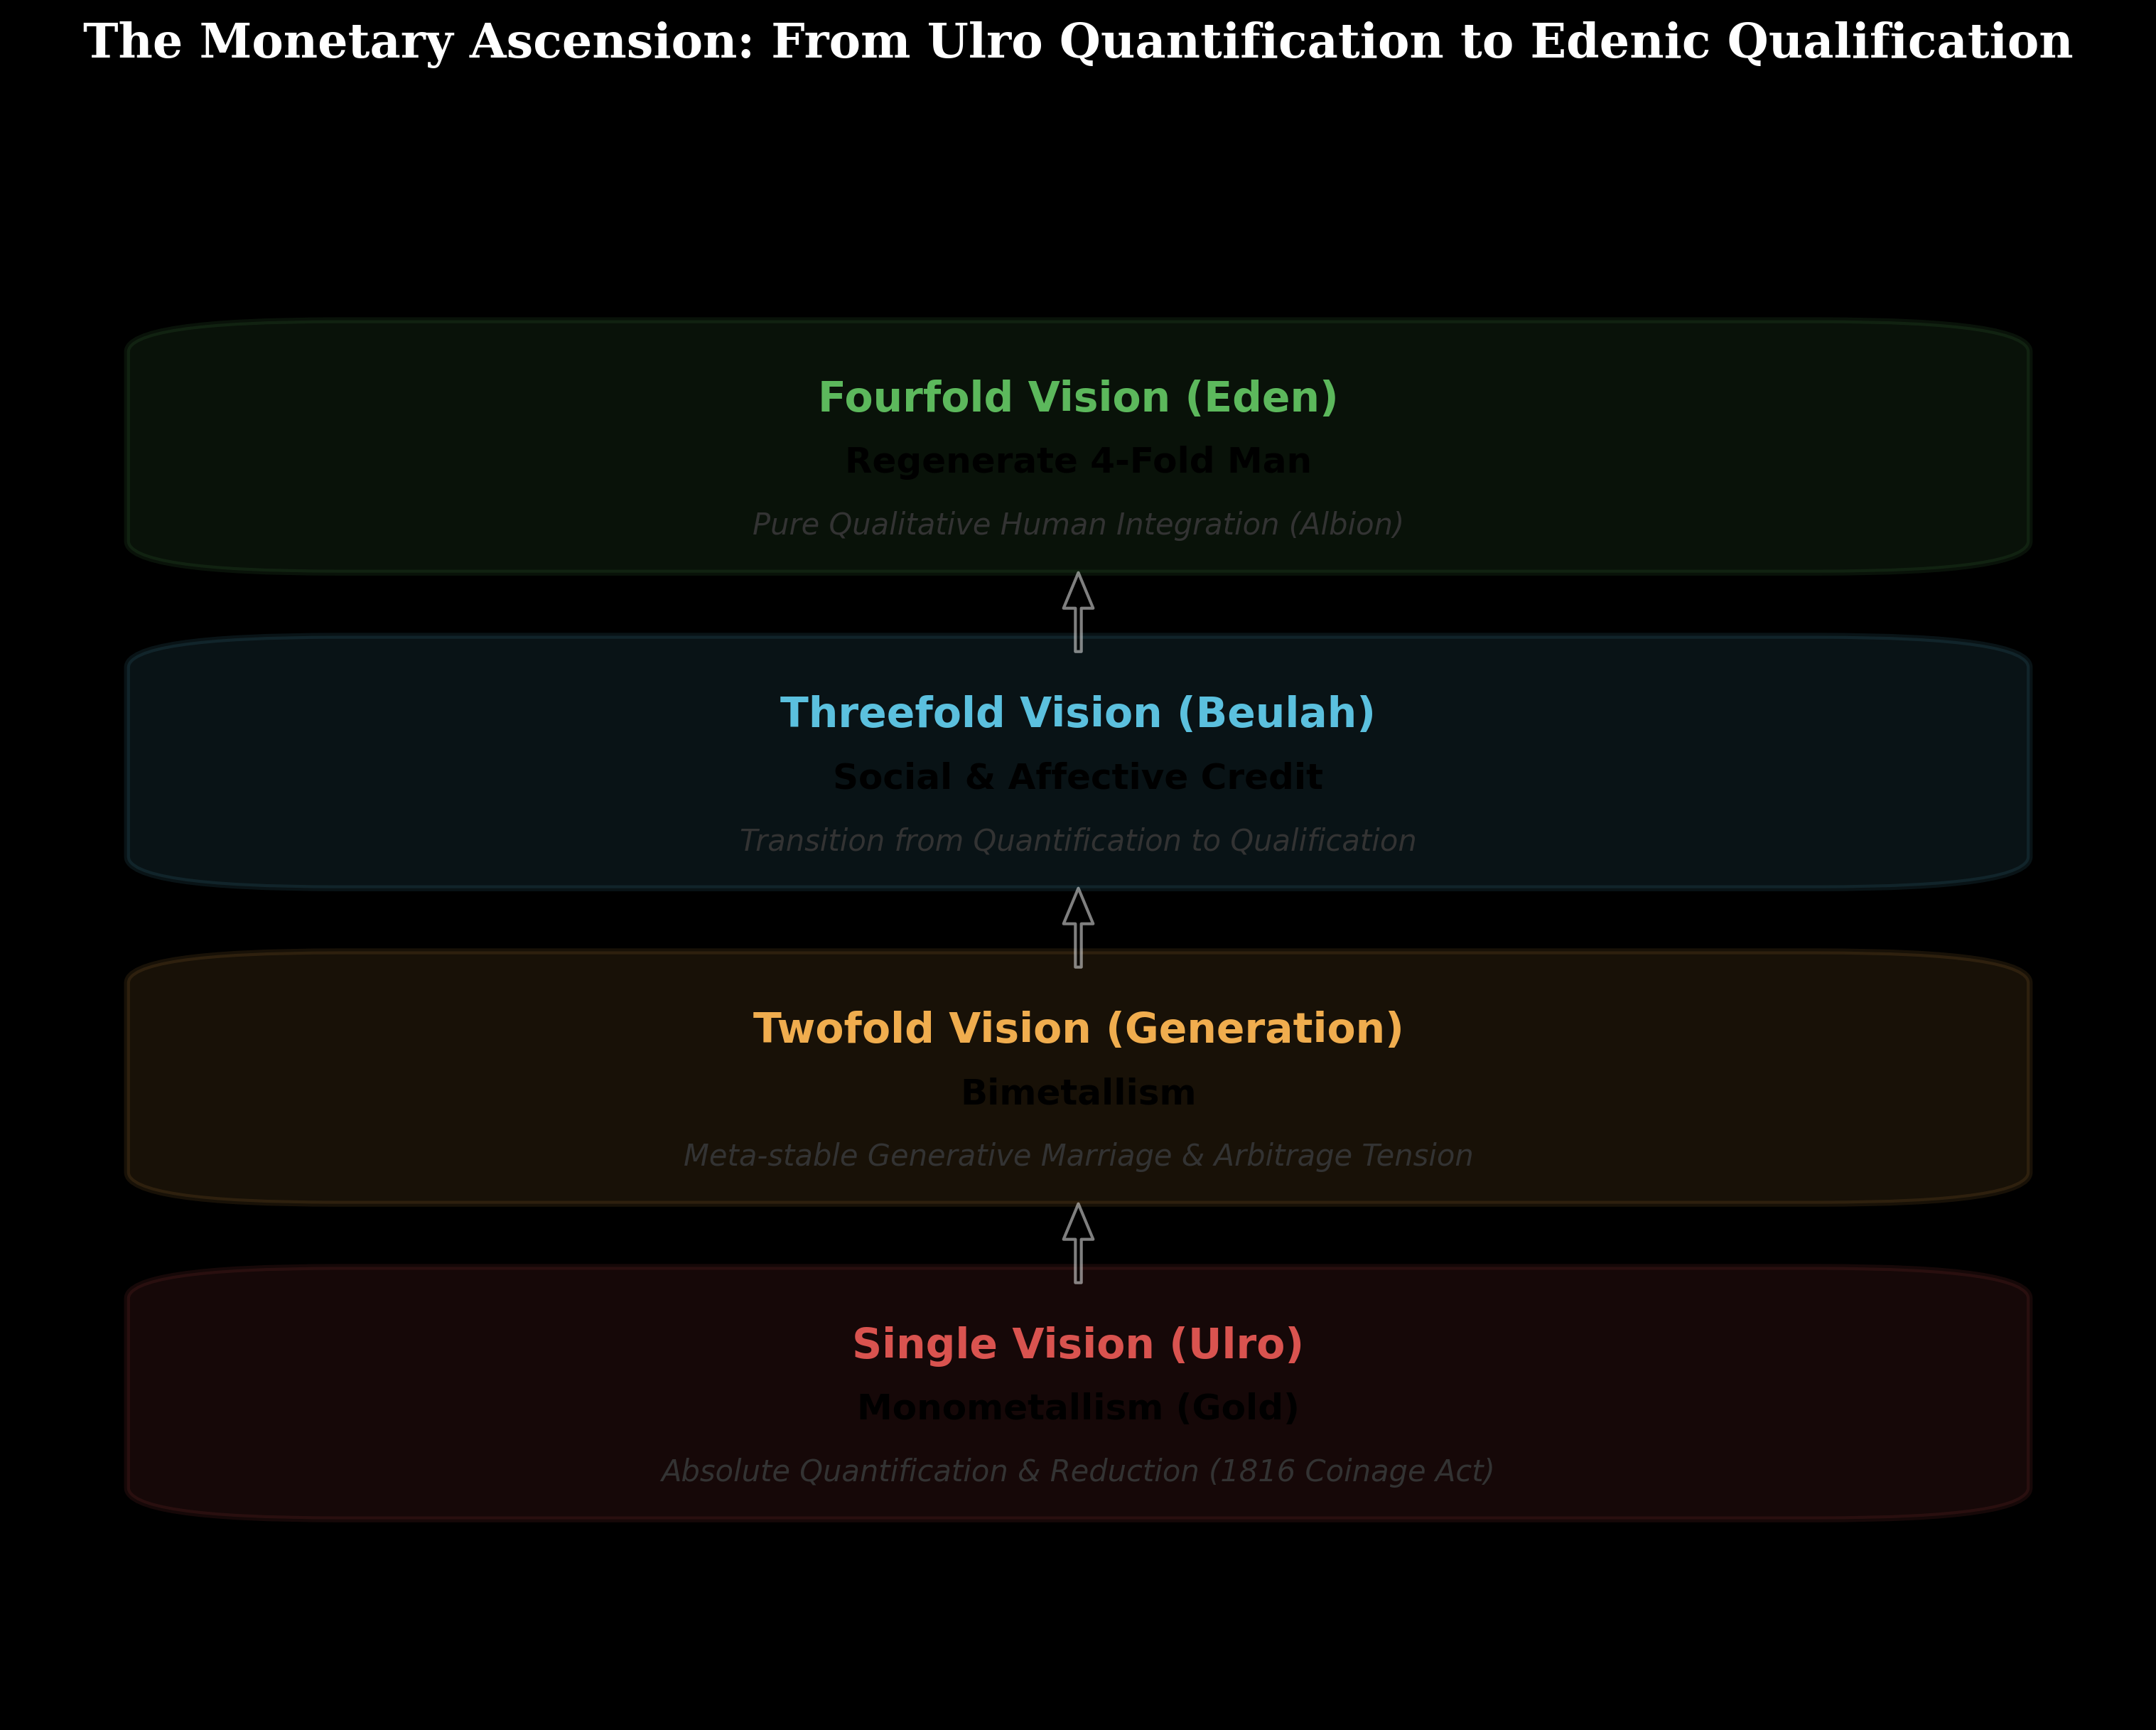
\includegraphics[keepaspectratio,alt={The Monetary Ascension --- From Ulro to Eden. A four-tiered ontological mapping elevating from the reductionist Monometallic standard of Ulro (Single Vision) through the generative bimetallic tension of Generation (Twofold Vision), the affective threshold of Beulah (Threefold Vision), and culminating in the non-dual qualitative integration of the Edenic state (Fourfold Vision). Each tier maps directly onto a specific historical monetary regime, from the sterile finality of the 1816 Gold Standard (Ulro) to the visionary artisanal economics embodied in Los's forge (Eden). This progression provides a critical topological heuristic for reading Blake's late epics: the journey out of the fallen world is not an escape from materiality, but an ascension through increasingly complex architectures of socio-economic relationality.}]{../figures/fourfold_mapping.png}}
\caption{The Monetary Ascension --- From Ulro to Eden. A four-tiered
ontological mapping elevating from the reductionist Monometallic
standard of Ulro (Single Vision) through the generative bimetallic
tension of Generation (Twofold Vision), the affective threshold of
Beulah (Threefold Vision), and culminating in the non-dual qualitative
integration of the Edenic state (Fourfold Vision). Each tier maps
directly onto a specific historical monetary regime, from the sterile
finality of the 1816 Gold Standard (Ulro) to the visionary artisanal
economics embodied in Los's forge (Eden). This progression provides a
critical topological heuristic for reading Blake's late epics: the
journey out of the fallen world is not an escape from materiality, but
an ascension through increasingly complex architectures of
socio-economic relationality.}\label{fig-fourfold}
\end{figure}
\end{block}
\end{frame}

\end{document}
